\documentclass[]{book}
\usepackage{lmodern}
\usepackage{amssymb,amsmath}
\usepackage{ifxetex,ifluatex}
\usepackage{fixltx2e} % provides \textsubscript
\ifnum 0\ifxetex 1\fi\ifluatex 1\fi=0 % if pdftex
  \usepackage[T1]{fontenc}
  \usepackage[utf8]{inputenc}
\else % if luatex or xelatex
  \ifxetex
    \usepackage{mathspec}
  \else
    \usepackage{fontspec}
  \fi
  \defaultfontfeatures{Ligatures=TeX,Scale=MatchLowercase}
\fi
% use upquote if available, for straight quotes in verbatim environments
\IfFileExists{upquote.sty}{\usepackage{upquote}}{}
% use microtype if available
\IfFileExists{microtype.sty}{%
\usepackage{microtype}
\UseMicrotypeSet[protrusion]{basicmath} % disable protrusion for tt fonts
}{}
\usepackage[margin=1in]{geometry}
\usepackage{hyperref}
\hypersetup{unicode=true,
            pdftitle={DRAFT Book Reproducible Templates},
            pdfauthor={Melinda K. Higgins},
            pdfborder={0 0 0},
            breaklinks=true}
\urlstyle{same}  % don't use monospace font for urls
\usepackage{natbib}
\bibliographystyle{apalike}
\usepackage{longtable,booktabs}
\usepackage{graphicx,grffile}
\makeatletter
\def\maxwidth{\ifdim\Gin@nat@width>\linewidth\linewidth\else\Gin@nat@width\fi}
\def\maxheight{\ifdim\Gin@nat@height>\textheight\textheight\else\Gin@nat@height\fi}
\makeatother
% Scale images if necessary, so that they will not overflow the page
% margins by default, and it is still possible to overwrite the defaults
% using explicit options in \includegraphics[width, height, ...]{}
\setkeys{Gin}{width=\maxwidth,height=\maxheight,keepaspectratio}
\IfFileExists{parskip.sty}{%
\usepackage{parskip}
}{% else
\setlength{\parindent}{0pt}
\setlength{\parskip}{6pt plus 2pt minus 1pt}
}
\setlength{\emergencystretch}{3em}  % prevent overfull lines
\providecommand{\tightlist}{%
  \setlength{\itemsep}{0pt}\setlength{\parskip}{0pt}}
\setcounter{secnumdepth}{5}
% Redefines (sub)paragraphs to behave more like sections
\ifx\paragraph\undefined\else
\let\oldparagraph\paragraph
\renewcommand{\paragraph}[1]{\oldparagraph{#1}\mbox{}}
\fi
\ifx\subparagraph\undefined\else
\let\oldsubparagraph\subparagraph
\renewcommand{\subparagraph}[1]{\oldsubparagraph{#1}\mbox{}}
\fi

%%% Use protect on footnotes to avoid problems with footnotes in titles
\let\rmarkdownfootnote\footnote%
\def\footnote{\protect\rmarkdownfootnote}

%%% Change title format to be more compact
\usepackage{titling}

% Create subtitle command for use in maketitle
\newcommand{\subtitle}[1]{
  \posttitle{
    \begin{center}\large#1\end{center}
    }
}

\setlength{\droptitle}{-2em}
  \title{DRAFT Book Reproducible Templates}
  \pretitle{\vspace{\droptitle}\centering\huge}
  \posttitle{\par}
  \author{Melinda K. Higgins}
  \preauthor{\centering\large\emph}
  \postauthor{\par}
  \predate{\centering\large\emph}
  \postdate{\par}
  \date{2018-01-20}

\usepackage{booktabs}
\usepackage{makeidx}
\makeindex
\usepackage[nottoc]{tocbibind}

\usepackage{amsthm}
\newtheorem{theorem}{Theorem}[chapter]
\newtheorem{lemma}{Lemma}[chapter]
\theoremstyle{definition}
\newtheorem{definition}{Definition}[chapter]
\newtheorem{corollary}{Corollary}[chapter]
\newtheorem{proposition}{Proposition}[chapter]
\theoremstyle{definition}
\newtheorem{example}{Example}[chapter]
\theoremstyle{definition}
\newtheorem{exercise}{Exercise}[chapter]
\theoremstyle{remark}
\newtheorem*{remark}{Remark}
\newtheorem*{solution}{Solution}
\begin{document}
\maketitle

{
\setcounter{tocdepth}{1}
\tableofcontents
}
\listoftables
\listoffigures
\chapter*{Preface}\label{preface}
\addcontentsline{toc}{chapter}{Preface}

aaaaaaaaaaaa

\section*{Why read this book}\label{why-read-this-book}
\addcontentsline{toc}{section}{Why read this book}

aaaaaaaaaaaaa

\section*{Structure of the book}\label{structure-of-the-book}
\addcontentsline{toc}{section}{Structure of the book}

aaaaaaaaaaaaaaaa

\section*{Software information and
conventions}\label{software-information-and-conventions}
\addcontentsline{toc}{section}{Software information and conventions}

aaaaaaaaaaaaaaaa

\section*{Acknowledgments}\label{acknowledgments}
\addcontentsline{toc}{section}{Acknowledgments}

aaaaaaaaaaaaaaa

\section*{Prerequisites}\label{prerequisites}
\addcontentsline{toc}{section}{Prerequisites}

This is a \emph{sample} book written in \textbf{Markdown}. You can use
anything that Pandoc's Markdown supports, e.g., a math equation
\(a^2 + b^2 = c^2\).

The \textbf{bookdown} package can be installed from CRAN or Github:

Remember each Rmd file contains one and only one chapter, and a chapter
is defined by the first-level heading \texttt{\#}.

To compile this example to PDF, you need to install XeLaTeX.

\section*{Colophon}\label{colophon}
\addcontentsline{toc}{section}{Colophon}

\subsection*{R Packages Used in This
Book}\label{r-packages-used-in-this-book}
\addcontentsline{toc}{subsection}{R Packages Used in This Book}

This book will use the \texttt{R} programming language \citep{R-base}
with the following \texttt{R} packages:

\begin{enumerate}
\def\labelenumi{\arabic{enumi}.}
\tightlist
\item
  \texttt{bookdown} \citep{R-bookdown}
\item
  \texttt{rmarkdown} \citep{R-rmarkdown}
\item
  \texttt{knitr} \citep{R-knitr}
\item
  \texttt{dplyr} \citep{R-dplyr}
\item
  \texttt{ggplot2} \citep{R-ggplot2}
\item
  \texttt{printr} \citep{R-printr}
\item
  \texttt{fivethirtyeight} \citep{R-fivethirtyeight}
\end{enumerate}

Other external refs, book \citep{xie2015}, and the FAD ref
\citep{Miller_Epstein_Bishop_Keitner_1985}.

\subsection*{R Session Info as of 2018-01-20
08:03:37}\label{r-session-info-as-of-2018-01-20-080337}
\addcontentsline{toc}{subsection}{R Session Info as of 2018-01-20
08:03:37}

This book was compiled using the \texttt{R} packages \texttt{bookdown},
\texttt{rmarkdown}, and \texttt{knitr} running under the following
\texttt{sessionInfo()}:

\begin{verbatim}
## R version 3.4.3 (2017-11-30)
## Platform: x86_64-w64-mingw32/x64 (64-bit)
## Running under: Windows 10 x64 (build 15063)
## 
## Matrix products: default
## 
## locale:
## [1] LC_COLLATE=English_United States.1252 
## [2] LC_CTYPE=English_United States.1252   
## [3] LC_MONETARY=English_United States.1252
## [4] LC_NUMERIC=C                          
## [5] LC_TIME=English_United States.1252    
## 
## attached base packages:
## [1] stats     graphics  grDevices utils     datasets  methods   base     
## 
## other attached packages:
## [1] fivethirtyeight_0.3.0 printr_0.1            ggplot2_2.2.1        
## [4] dplyr_0.7.4           knitr_1.18            rmarkdown_1.8.5      
## [7] bookdown_0.5.10      
## 
## loaded via a namespace (and not attached):
##  [1] Rcpp_0.12.13     rstudioapi_0.7   bindr_0.1        magrittr_1.5    
##  [5] munsell_0.4.3    colorspace_1.3-2 R6_2.2.2         rlang_0.1.4     
##  [9] plyr_1.8.4       stringr_1.2.0    tools_3.4.3      grid_3.4.3      
## [13] gtable_0.2.0     htmltools_0.3.6  lazyeval_0.2.0   yaml_2.1.16     
## [17] rprojroot_1.3-2  digest_0.6.12    assertthat_0.2.0 tibble_1.3.4    
## [21] bindrcpp_0.2     glue_1.1.1       evaluate_0.10.1  stringi_1.1.5   
## [25] compiler_3.4.3   scales_0.5.0     backports_1.1.1  pkgconfig_2.0.1
\end{verbatim}

\chapter*{About the Author}\label{about-the-author}
\addcontentsline{toc}{chapter}{About the Author}

Melinda Higgins has dual degrees in Chemometrics (PhD) and Statistics
(MS) with 25 years experience in research, teaching, consulting,
directing and managing projects. Her expertise includes
programming/scripting languages (R, S, Pascal, Perl, Prolog) and
statistical, mathematical, imaging, and geo-spatial processing software
packages (R, SAS, SPSS, MATLAB, SYSTAT, ENVI, ESRI ArcView, IMAGINE).
While at Georgia Tech Research Institute (1994-2011), she coordinated
large team projects with rigorous timelines, milestone tracking and
version control in the areas of remote sensing, geospatial information
systems, sensor fusion and target recognition. In her current work at
Emory (2007 --), she has 10+ yr expertise mentoring students and faculty
in nursing and public health science research and scholarship. Her
health research experience includes pattern recognition, phenotype
characterizations and longitudinal modeling in heart failure, diabetes,
cognitive impairment, and HIV/AIDS chronic disease populations.

\part{Part One}\label{part-part-one}

\chapter{Introduction}\label{intro}

You can label chapter and section titles using \texttt{\{\#label\}}
after them, e.g., we can reference Chapter \ref{intro}. If you do not
manually label them, there will be automatic labels anyway, e.g.,
Chapter \ref{methods}.

Figures and tables with captions will be placed in \texttt{figure} and
\texttt{table} environments, respectively.

\begin{figure}

{\centering 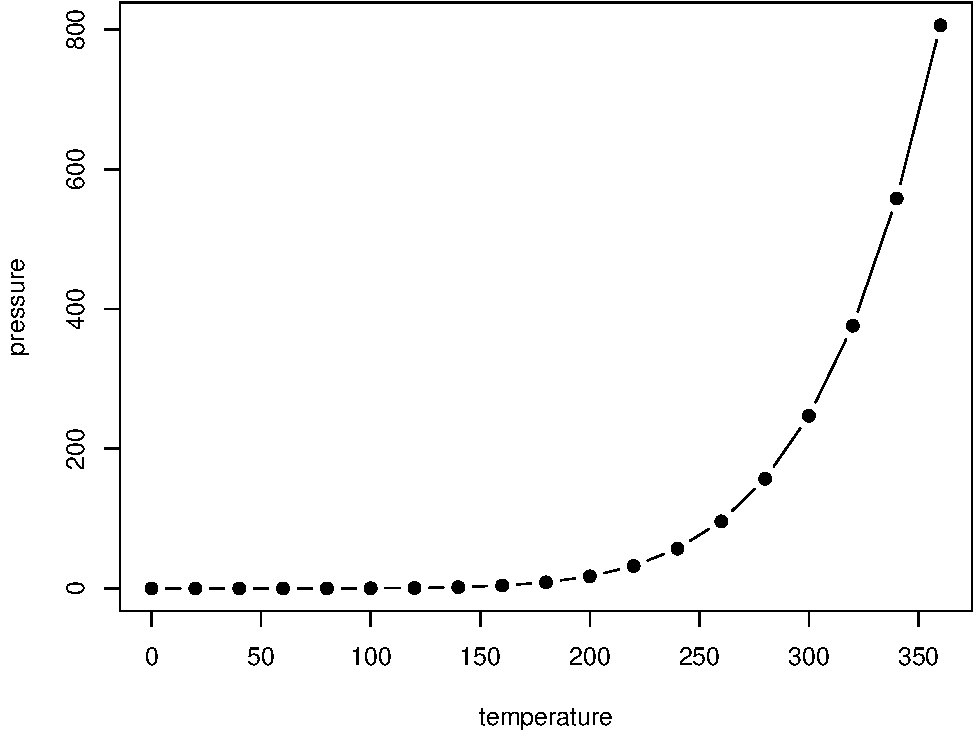
\includegraphics[width=0.8\linewidth]{BookRepTemplates_files/figure-latex/nice-fig-1} 

}

\caption{Here is a nice figure!}\label{fig:nice-fig}
\end{figure}

Reference a figure by its code chunk label with the \texttt{fig:}
prefix, e.g., see Figure \ref{fig:nice-fig}. Similarly, you can
reference tables generated from \texttt{knitr::kable()}, e.g., see Table
\ref{tab:nice-tab}.

\begin{table}

\caption{\label{tab:nice-tab}Here is a nice table!}
\centering
\begin{tabular}[t]{rrrrl}
\toprule
Sepal.Length & Sepal.Width & Petal.Length & Petal.Width & Species\\
\midrule
5.1 & 3.5 & 1.4 & 0.2 & setosa\\
4.9 & 3.0 & 1.4 & 0.2 & setosa\\
4.7 & 3.2 & 1.3 & 0.2 & setosa\\
4.6 & 3.1 & 1.5 & 0.2 & setosa\\
5.0 & 3.6 & 1.4 & 0.2 & setosa\\
\addlinespace
5.4 & 3.9 & 1.7 & 0.4 & setosa\\
4.6 & 3.4 & 1.4 & 0.3 & setosa\\
5.0 & 3.4 & 1.5 & 0.2 & setosa\\
4.4 & 2.9 & 1.4 & 0.2 & setosa\\
4.9 & 3.1 & 1.5 & 0.1 & setosa\\
\addlinespace
5.4 & 3.7 & 1.5 & 0.2 & setosa\\
4.8 & 3.4 & 1.6 & 0.2 & setosa\\
4.8 & 3.0 & 1.4 & 0.1 & setosa\\
4.3 & 3.0 & 1.1 & 0.1 & setosa\\
5.8 & 4.0 & 1.2 & 0.2 & setosa\\
\addlinespace
5.7 & 4.4 & 1.5 & 0.4 & setosa\\
5.4 & 3.9 & 1.3 & 0.4 & setosa\\
5.1 & 3.5 & 1.4 & 0.3 & setosa\\
5.7 & 3.8 & 1.7 & 0.3 & setosa\\
5.1 & 3.8 & 1.5 & 0.3 & setosa\\
\bottomrule
\end{tabular}
\end{table}

You can write citations, too. For example, we are using the
\textbf{bookdown} \index{bookdown} package \citep{R-bookdown} in this
sample book, which was built on top of R Markdown \index{R Markdown} and
\textbf{knitr} \index{knitr} \citep{xie2015}.

\chapter{Literature}\label{literature}

Here is a review of existing methods.

\part{Part Two}\label{part-part-two}

\chapter{Methods}\label{methods}

We describe our methods \index{Some Methods} in this chapter.

add more random text \index{text}.

\chapter{Applications}\label{applications}

Some \emph{significant} applications are demonstrated in this chapter.

\section{Example one}\label{example-one}

\section{Example two}\label{example-two}

\chapter{Final Words}\label{final-words}

We have finished a nice book \index{Nice Book}.

some random \index{random} text

\part{Appendix}\label{part-appendix}

\appendix


\chapter{First appendix section}\label{first-appendix-section}

We have finished a nice book \index{Nice Book}.

some random \index{random} text

\chapter{another appendix section}\label{another-appendix-section}

We have finished a nice book \index{Nice Book}.

some random \index{random} text

\bibliography{book.bib,packages.bib}

\printindex


\end{document}
